\subsubsection{21.11.14 (Competition)}

\begin{center}
	1-nd day of competition "Robofest-South"
\end{center}
Today there was training matches.\newline

Improvements that were done:
\begin{enumerate}
	\item It was turned out that robot loses clutch with the floor when small ball gets under the wheel. To prevent this it was installed protection of wheels from the balls.
	
	\begin{figure}[H]
		\begin{minipage}[h]{0.2\linewidth}
			\center  
		\end{minipage}
		\begin{minipage}[h]{0.6\linewidth}
			\center{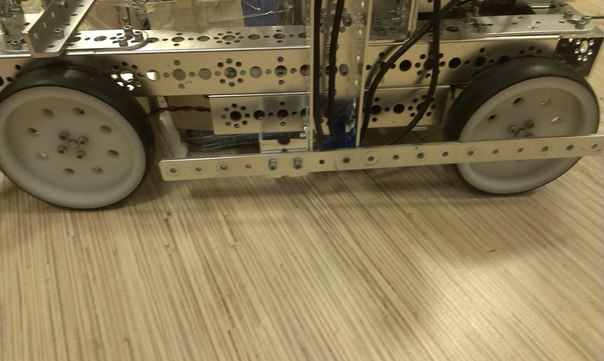
\includegraphics[scale=0.3]{days/21.11.14/images/01}}
			\caption{Protection of wheels from the balls}
		\end{minipage}
	\end{figure}
	
	\item It was turned out that base of rolling goal does not pass under the bottom of the robot. It doesn't allow to bring the goal as close as possible to the robot. To correct this problem it was decided to increase clearance of back part of robot turning the motors in their mounts so that shaft was on the bottom.
	
	\item Beams on the MCB was sawed to needed length and were fixed. But due to problems with servo ,that shore the beams, MCB was changed. Faulty servo was removed and beams were fixed rigidly.
	\begin{figure}[H]
		\begin{minipage}[h]{0.2\linewidth}
			\center  
		\end{minipage}
		\begin{minipage}[h]{0.6\linewidth}
			\center{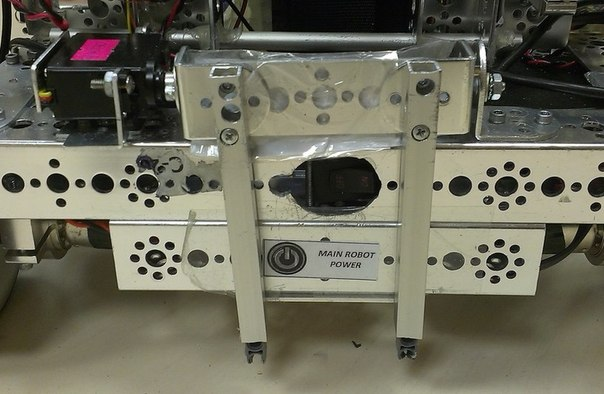
\includegraphics[scale=0.3]{days/21.11.14/images/02}}
			\caption{Changed MCB}
		\end{minipage}
	\end{figure}
	
	\item It was installed Samanta-module and it was conducted one training match on the field for competitions.
	
	\begin{figure}[H]
		\begin{minipage}[h]{1\linewidth}
			\center{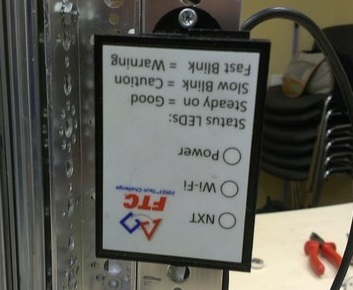
\includegraphics[scale=0.4]{days/21.11.14/images/03}}
		\end{minipage}
		\caption{Mount of Samanta}
	\end{figure}
	 	
\end{enumerate}
\fillpage